\scanpage{168}
\mspage{23}
on a pu obtenir via fppf un $H^1$ correct, alors que pour le $H^2$ déjà tous les essais \unsure{ont|nt} été infructueux.

À vrai dire, on conjecture que \uline{toute} la partie de pente $\leq 1$ du $H^i_{\mathrm{cris}}$ provient de fppf : Mais j'ai perdu complètement contact avec ces questions -- des gens comme Mazur, Katz, Messing -- et bien sûr, Deligne -- devraient être au courant du point où en est la question.\unsure{.}

\figure{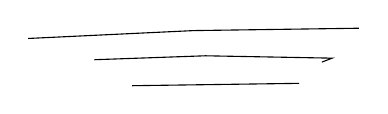
\begin{tikzpicture}[x=1cm,y=1cm]
\draw (0,0) -- (2.1,.10) -- (4.2,.13);
\draw (.84,-.27) -- (2.25,-.22) -- (3.86,-.25) -- (3.73,-.30);
\draw (1.32,-.60) -- (3.44,-.57);
\end{tikzpicture}}

Ta question $7^{\circ}$ semble indiquer qu'il y a malentendu en ton esprit sur la signification du ``type d'homotopie'' de $X$, $X$ un topos (p.ex. le topos \unsure{étale|étal} d'un schéma). Sans doute tu dois confondre l'\unsure{algèbre|algebre} homotopique qu'on peut faire sur $X$ à coups de faisceaux semi-simpliciaux, de champs en \unsure{tous|tout} \unsure{genre|genres}, et des relations entre ceux-ci -- et cet autre point de vue où $X$ (avec sa structure si riche de topos) \unsure{disparait|disparaît} virtuellement,
% archive sheet number: 168
